% Sensor Comparison Figure (CO2 vs Gas Resistance)
% Include with: % Sensor Comparison Figure (CO2 vs Gas Resistance)
% Include with: % Sensor Comparison Figure (CO2 vs Gas Resistance)
% Include with: % Sensor Comparison Figure (CO2 vs Gas Resistance)
% Include with: \input{figures/sensor_comparison.tex}
% Requires: \usepackage{pgfplots}

\begin{figure}[ht]
\centering
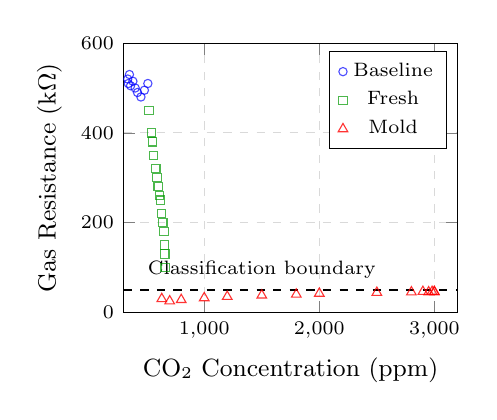
\begin{tikzpicture}
\begin{axis}[
    width=0.48\textwidth,
    height=5cm,
    xlabel={CO\textsubscript{2} Concentration (ppm)},
    ylabel={Gas Resistance (k$\Omega$)},
    xmin=300, xmax=3200,
    ymin=0, ymax=600,
    legend pos=north east,
    legend style={font=\scriptsize},
    grid=major,
    grid style={dashed, gray!30},
    tick label style={font=\scriptsize},
    label style={font=\small},
]

% Baseline cluster (low CO2, high resistance)
\addplot[only marks, mark=o, mark size=1.5pt, blue, opacity=0.7]
    coordinates {
        (335, 520) (340, 510) (350, 530) (360, 505) (380, 515)
        (400, 500) (420, 490) (450, 480) (480, 495) (510, 510)
    };
\addlegendentry{Baseline}

% Fresh fruit cluster (medium CO2, variable resistance)
\addplot[only marks, mark=square, mark size=1.5pt, green!60!black, opacity=0.7]
    coordinates {
        (520, 450) (550, 380) (580, 320) (600, 280) (620, 250)
        (640, 200) (650, 180) (655, 150) (658, 130) (660, 100)
        (540, 400) (560, 350) (590, 300) (610, 260) (630, 220)
    };
\addlegendentry{Fresh}

% Mold cluster (high CO2, very low resistance)
\addplot[only marks, mark=triangle, mark size=2pt, red, opacity=0.8]
    coordinates {
        (631, 30) (700, 25) (800, 28) (1000, 32) (1200, 35)
        (1500, 38) (1800, 40) (2000, 42) (2500, 44) (2800, 45)
        (2900, 46) (2950, 45) (2980, 46) (2999, 46) (3000, 45)
    };
\addlegendentry{Mold}

% Decision boundary approximation
\addplot[dashed, black, thick, domain=300:3200] {50};
\node[font=\scriptsize, anchor=south] at (axis cs:1500,55) {Classification boundary};

\end{axis}
\end{tikzpicture}
\caption{Sensor fusion for spoilage classification. Fresh and mold states are clearly separable in the CO\textsubscript{2}--Gas Resistance feature space. The mold cluster (red triangles) shows characteristically low gas resistance ($<$50\,k$\Omega$) combined with elevated CO\textsubscript{2} levels reaching sensor saturation at 3000\,ppm.}
\label{fig:sensor_comparison}
\end{figure}

% Requires: \usepackage{pgfplots}

\begin{figure}[ht]
\centering
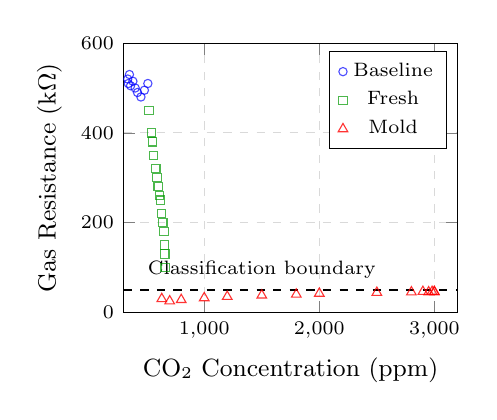
\begin{tikzpicture}
\begin{axis}[
    width=0.48\textwidth,
    height=5cm,
    xlabel={CO\textsubscript{2} Concentration (ppm)},
    ylabel={Gas Resistance (k$\Omega$)},
    xmin=300, xmax=3200,
    ymin=0, ymax=600,
    legend pos=north east,
    legend style={font=\scriptsize},
    grid=major,
    grid style={dashed, gray!30},
    tick label style={font=\scriptsize},
    label style={font=\small},
]

% Baseline cluster (low CO2, high resistance)
\addplot[only marks, mark=o, mark size=1.5pt, blue, opacity=0.7]
    coordinates {
        (335, 520) (340, 510) (350, 530) (360, 505) (380, 515)
        (400, 500) (420, 490) (450, 480) (480, 495) (510, 510)
    };
\addlegendentry{Baseline}

% Fresh fruit cluster (medium CO2, variable resistance)
\addplot[only marks, mark=square, mark size=1.5pt, green!60!black, opacity=0.7]
    coordinates {
        (520, 450) (550, 380) (580, 320) (600, 280) (620, 250)
        (640, 200) (650, 180) (655, 150) (658, 130) (660, 100)
        (540, 400) (560, 350) (590, 300) (610, 260) (630, 220)
    };
\addlegendentry{Fresh}

% Mold cluster (high CO2, very low resistance)
\addplot[only marks, mark=triangle, mark size=2pt, red, opacity=0.8]
    coordinates {
        (631, 30) (700, 25) (800, 28) (1000, 32) (1200, 35)
        (1500, 38) (1800, 40) (2000, 42) (2500, 44) (2800, 45)
        (2900, 46) (2950, 45) (2980, 46) (2999, 46) (3000, 45)
    };
\addlegendentry{Mold}

% Decision boundary approximation
\addplot[dashed, black, thick, domain=300:3200] {50};
\node[font=\scriptsize, anchor=south] at (axis cs:1500,55) {Classification boundary};

\end{axis}
\end{tikzpicture}
\caption{Sensor fusion for spoilage classification. Fresh and mold states are clearly separable in the CO\textsubscript{2}--Gas Resistance feature space. The mold cluster (red triangles) shows characteristically low gas resistance ($<$50\,k$\Omega$) combined with elevated CO\textsubscript{2} levels reaching sensor saturation at 3000\,ppm.}
\label{fig:sensor_comparison}
\end{figure}

% Requires: \usepackage{pgfplots}

\begin{figure}[ht]
\centering
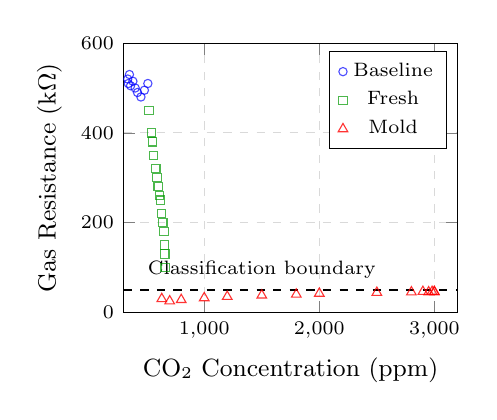
\begin{tikzpicture}
\begin{axis}[
    width=0.48\textwidth,
    height=5cm,
    xlabel={CO\textsubscript{2} Concentration (ppm)},
    ylabel={Gas Resistance (k$\Omega$)},
    xmin=300, xmax=3200,
    ymin=0, ymax=600,
    legend pos=north east,
    legend style={font=\scriptsize},
    grid=major,
    grid style={dashed, gray!30},
    tick label style={font=\scriptsize},
    label style={font=\small},
]

% Baseline cluster (low CO2, high resistance)
\addplot[only marks, mark=o, mark size=1.5pt, blue, opacity=0.7]
    coordinates {
        (335, 520) (340, 510) (350, 530) (360, 505) (380, 515)
        (400, 500) (420, 490) (450, 480) (480, 495) (510, 510)
    };
\addlegendentry{Baseline}

% Fresh fruit cluster (medium CO2, variable resistance)
\addplot[only marks, mark=square, mark size=1.5pt, green!60!black, opacity=0.7]
    coordinates {
        (520, 450) (550, 380) (580, 320) (600, 280) (620, 250)
        (640, 200) (650, 180) (655, 150) (658, 130) (660, 100)
        (540, 400) (560, 350) (590, 300) (610, 260) (630, 220)
    };
\addlegendentry{Fresh}

% Mold cluster (high CO2, very low resistance)
\addplot[only marks, mark=triangle, mark size=2pt, red, opacity=0.8]
    coordinates {
        (631, 30) (700, 25) (800, 28) (1000, 32) (1200, 35)
        (1500, 38) (1800, 40) (2000, 42) (2500, 44) (2800, 45)
        (2900, 46) (2950, 45) (2980, 46) (2999, 46) (3000, 45)
    };
\addlegendentry{Mold}

% Decision boundary approximation
\addplot[dashed, black, thick, domain=300:3200] {50};
\node[font=\scriptsize, anchor=south] at (axis cs:1500,55) {Classification boundary};

\end{axis}
\end{tikzpicture}
\caption{Sensor fusion for spoilage classification. Fresh and mold states are clearly separable in the CO\textsubscript{2}--Gas Resistance feature space. The mold cluster (red triangles) shows characteristically low gas resistance ($<$50\,k$\Omega$) combined with elevated CO\textsubscript{2} levels reaching sensor saturation at 3000\,ppm.}
\label{fig:sensor_comparison}
\end{figure}

% Requires: \usepackage{pgfplots}

\begin{figure}[ht]
\centering
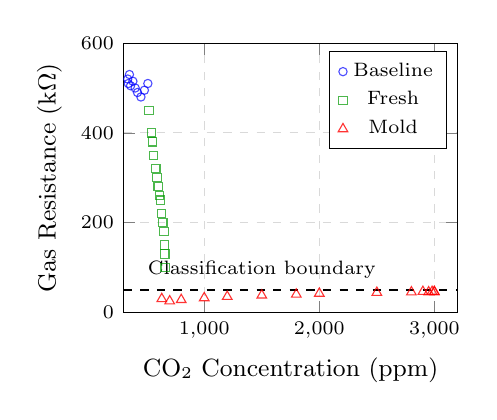
\begin{tikzpicture}
\begin{axis}[
    width=0.48\textwidth,
    height=5cm,
    xlabel={CO\textsubscript{2} Concentration (ppm)},
    ylabel={Gas Resistance (k$\Omega$)},
    xmin=300, xmax=3200,
    ymin=0, ymax=600,
    legend pos=north east,
    legend style={font=\scriptsize},
    grid=major,
    grid style={dashed, gray!30},
    tick label style={font=\scriptsize},
    label style={font=\small},
]

% Baseline cluster (low CO2, high resistance)
\addplot[only marks, mark=o, mark size=1.5pt, blue, opacity=0.7]
    coordinates {
        (335, 520) (340, 510) (350, 530) (360, 505) (380, 515)
        (400, 500) (420, 490) (450, 480) (480, 495) (510, 510)
    };
\addlegendentry{Baseline}

% Fresh fruit cluster (medium CO2, variable resistance)
\addplot[only marks, mark=square, mark size=1.5pt, green!60!black, opacity=0.7]
    coordinates {
        (520, 450) (550, 380) (580, 320) (600, 280) (620, 250)
        (640, 200) (650, 180) (655, 150) (658, 130) (660, 100)
        (540, 400) (560, 350) (590, 300) (610, 260) (630, 220)
    };
\addlegendentry{Fresh}

% Mold cluster (high CO2, very low resistance)
\addplot[only marks, mark=triangle, mark size=2pt, red, opacity=0.8]
    coordinates {
        (631, 30) (700, 25) (800, 28) (1000, 32) (1200, 35)
        (1500, 38) (1800, 40) (2000, 42) (2500, 44) (2800, 45)
        (2900, 46) (2950, 45) (2980, 46) (2999, 46) (3000, 45)
    };
\addlegendentry{Mold}

% Decision boundary approximation
\addplot[dashed, black, thick, domain=300:3200] {50};
\node[font=\scriptsize, anchor=south] at (axis cs:1500,55) {Classification boundary};

\end{axis}
\end{tikzpicture}
\caption{Sensor fusion for spoilage classification. Fresh and mold states are clearly separable in the CO\textsubscript{2}--Gas Resistance feature space. The mold cluster (red triangles) shows characteristically low gas resistance ($<$50\,k$\Omega$) combined with elevated CO\textsubscript{2} levels reaching sensor saturation at 3000\,ppm.}
\label{fig:sensor_comparison}
\end{figure}
